\chapter{Pravidla hry}
Logic je desková hra pro dva hráče. Jeden hráč určí hledanou kombinaci, dále bude označován jako hráč A, a druhý tuto kombinaci za pomocí logických úvah a
vyhodnocení hráčem A hledá, dále bude označován jako hráč B.

Hráči si určí herní pozice. Hráč A vybere barvy a následně je v určitém pořadí vloží do zadávacího pole a zakryje je, aby tuto
kombinaci spoluhráč neviděl. Hráč B je v této chvíli otočen. Hráč B následně zvolí náhodnou kombinaci barev a pozic. Po ukončení tahu nechá
hráče A, aby tah vyhodnotil. Hráč A vyhodnotí tah následujícím způsobem. Pokud hráč B vložil správnou barvu na správnou pozici, tak vloží 
do vyhodnocovací sekce černý kolík. Pokud vložil barvu, která se v zadání vyskytuje, ale vložil ji na nesprávnou pozici, tak vloží bílý kolík.
Pokud zůstanou některé pozice neobsazené, tak to znamená, že daná barva se v zadání nevyskytuje. Poté začne hráč B na základě vyhodnocení a 
svých všech předchozích tahů hledat kombinaci.

Cílem hry je nalézt správnou kombinaci dříve, než skončí plocha herního pole.

Těžší varianta spočívá v možnosti absence barvy - v zadání je mezera.

\chapter{Popis zapojení}

\section{Procesor}
Byl vybrán procesor ESP32-PICO-D4.

Tento procesor obsahuje \cite{PICO_datasheet}: %napsáno zatím pro WROOM - opravit
\begin{itemize}
    \item WiFi,
    \item Bluetooth,
    \item procesor,
    \item průměrný odběr proudu 80 mA,
    \item 32 GPIO pinů,
    \item dvoujádrový 32bitový procesor Xtensa LX6,
    \item 520 kB SRAM, %?
    \item 16 MB FLASH. %?
  \end{itemize}

  Napájecí napětí tohoto procesoru je od 3,0 do 3,6 V \cite{PICO_datasheet}. ESP32-PICO má vyvedeno 32 GPIO pinů, které je 
  možno softwarově nastavit jako vstupní nebo výstupní. Na tyto piny lze poté připojit různá zařízení. Vstupním senzorem může 
  být typicky tlačítko a výstupním indikátorem např. LED. Tato zařízení zprostředkovávají komunikaci mezi procesorem a okolním 
  světem.

  Zapojení pinu EN bylo převzato ze schématu \cite{PICO_datasheet}.

  GPIO piny IO16 a IO17 nemohou být použity, protože ESP32-PICO má na těchto pinech připojenou flash paměť \cite{PICO_datasheet}.
  Pokud by na tento pin bylo něco připojeno, tak by se procesor nedostal do své paměti. Nahraný program do procesoru by tedy
  nemohl být načten a DPS by ztratila svoji funkci.

  GPIO piny IO34 a vyšší jsou pouze vstupní \cite{PICO_datasheet}. Vstupní piny nemají softwarově zapojitelný pullup rezistor. 
  Pokud je tedy zapotřebí pullup rezistor, musí se fyzicky zapojit.
  
  \section{Napájení}
  \subsection{v0.0}
  \subsection{v1.0}
  Ve verzi 1.0 bylo napájení předěláno. Napájení v této verzi neprobíhá přes baterie, ale pouze přes USB konektor. Byl 
  zvolen konektor USB Micro.
  Výhody:
  \begin{itemize}
    \item Absence nabíjecího obvodu,
    \item absence hlídání stavu nabití baterie,
    \item absence ochrany proti přepólování (USB konektor je uzpůsoben svým tvarem, aby uživatel nemohl napájení přepólovat.),
    \item .
  \end{itemize}

  Nevýhody:
  \begin{itemize}
    \item Předpokládá se, že uživatel vlastní powerbanku.% vymyslet další
  \end{itemize}

  \section{Stepdown}
  Procesor ESP32-PICO-D4 má napájecí napětí 3,3 V. Napětí z powerbanky přes USB je 5 V. Proto je tedy zapotřebí zapojit 
  stepdown, který bude vytvářet napájecí napětí pro procesor.

  Jako stepdown byl zvolen čip SY8105.
  Parametry čipu SY8105 \cite{SY8105_datasheet}:
  \begin{itemize}
    \item Vstupní napětí 1,5 - 18 V,
    \item výstupní proud 5 A,
    \item pouzdro TSOT23-6.
  \end{itemize}

  \begin{figure}[!h]
    \begin{center}
      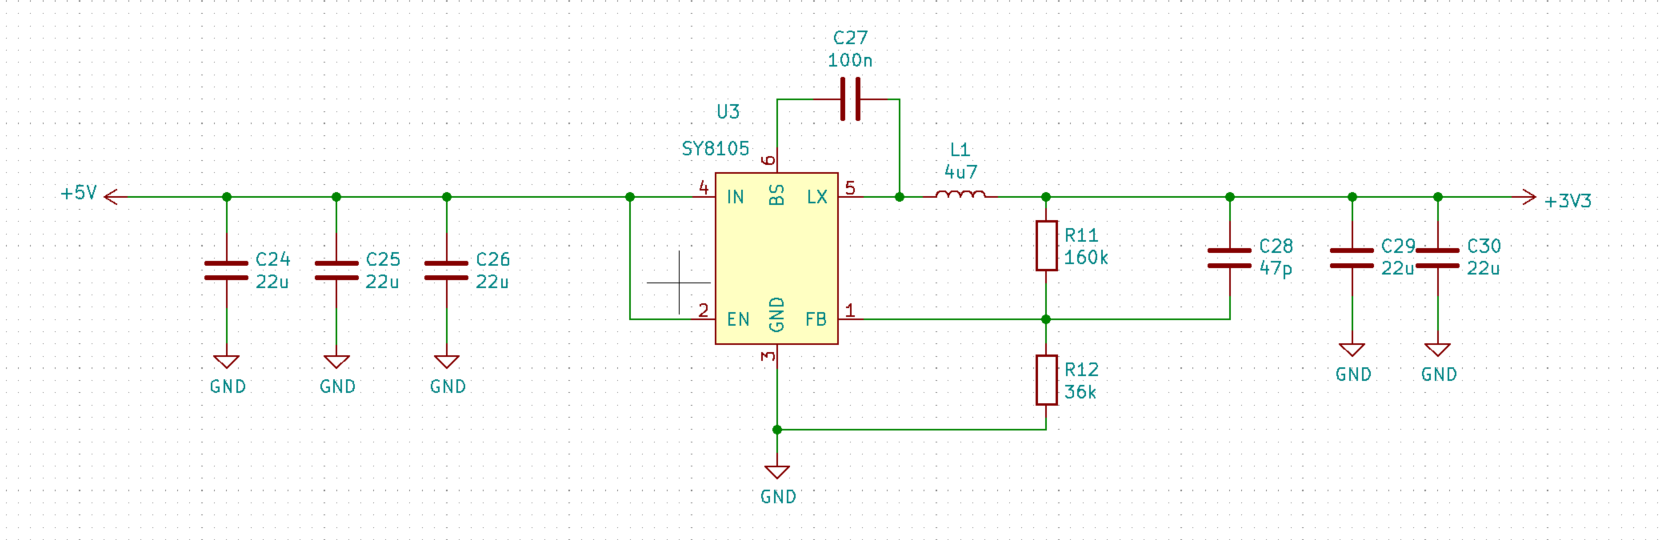
\includegraphics[scale=0.5]{obrazky/SY8105_schema.png}
    \end{center}
    \caption[SY8105 schéma]{Schéma zapojení čipu SY8105 \cite{SY8105_datasheet}.}
  \end{figure}

  Výstupní napětí je závislé na poměru odporů R11 a R12. Nastavené velikosti odporů jsou pro výstupní napětí 3,3 V pro procesor 
  ESP32-PICO.

  \section{Převodník z USB na RS-232}
  Procesor ESP32-PICO používá jako komunikační rozhraní linku RS-232. Programování ale probíhá přes USB, které toto rozhraní
  nemá. Proto bylo potřeba použít převodník z USB na rozhraní RS-232.
  
  Pro převod z USB na RS-232 byl použit čip CP2102, který  zároveň převádí logiku 0 - 5 V na logiku 0 - 3,3 V 
  \cite{CP2102_datasheet}. Tento čip byl vybrán z důvodu použití i na kitu ESP32-DEVKITC, kde je funkční.
  Zapojení čipu bylo převzato z tohoto kitu ESP32-DEVKITC.

  Čip CP2102 dokáže komunikovat vekým množstvím komunikačních rychlostí (300, 9600, 19200, 38400, 115200, 256000, atd) 
  \cite{CP2102_datasheet}. PC započne komunikaci určitou rychlostí a tento čip tuto komunikaci zachytí, určí rychlost 
  a touto rychlostí začne probíhat programování.

Parametry čipu CP2102 \cite{CP2102_datasheet}: %přidat
\begin{itemize}
    \item regulátor 3,3 V,
    \item typický odběr proudu 9,5 mA.
\end{itemize}

\begin{figure}[!h]
    \begin{center}
      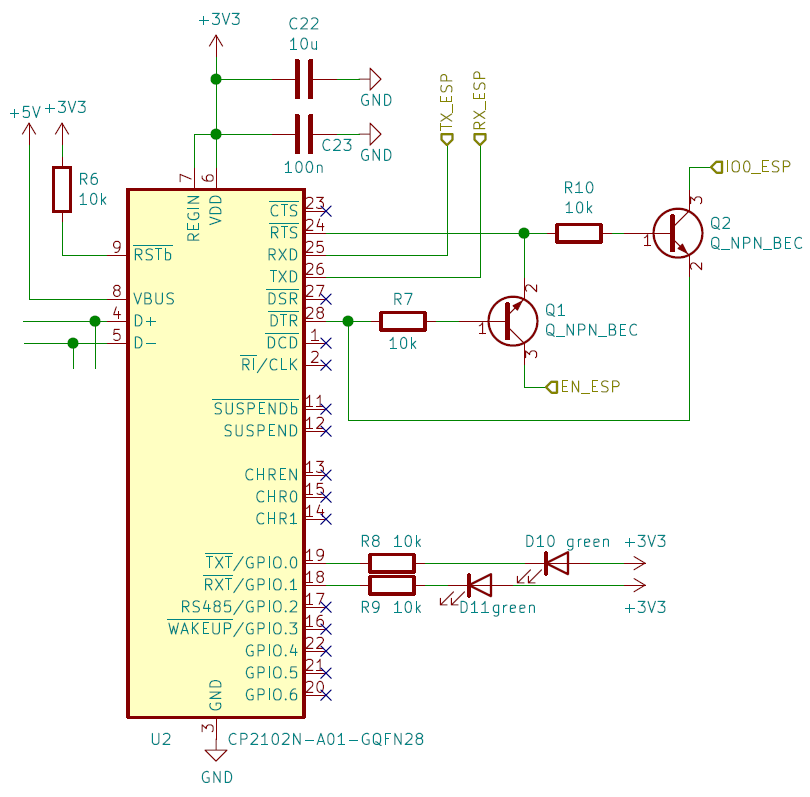
\includegraphics[scale=0.5]{obrazky/CP2102_schema.png}
    \end{center}
    \caption[CP2102 schéma]{Schéma zapojení převodníku z USB na RS-232 \cite{Devkit_schema}.}
\end{figure}

Z USB jsou signály D+ a D- připojeny k čipu CP2102. Tento čip tento signál převede na signály RX a TX, které mají výstup 
na pinech RXD a TXD. Následně jsou tyto signály připojeny k procesoru ESP32-PICO. Signály RX a TX se musí překřížit – RX 
CP2102 se připojí na TX ESP32-PICO a TX CP2102 se připojí na RX ESP32-PICO. 

LED D10 a D11 slouží k indikaci komunikace s procesorem. Jsou zapojeny podle datasheetu \cite{CP2102_datasheet}. Pokud je do 
procesoru nahráván program, tak LED D10 a D11 blikají.

\begin{figure}[!h]
    \begin{center}
      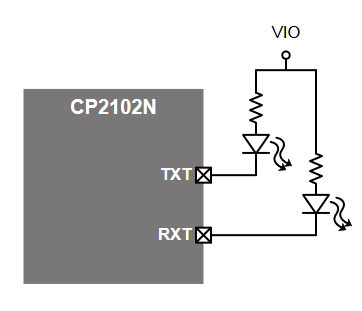
\includegraphics[scale=0.5]{obrazky/CP2102_LED.png}
    \end{center}
    \caption[CP2102 LED]{Zapojení LED pro indikaci komunikace s procesorem k čipu CP2102 \cite{CP2102_datasheet}.}
\end{figure}

\section{LED}
Byly vybrány LED typu WS2812C. Tento typ LED je určen pro přenosná zařízení, díky jejich nízké spotřebě. Tyto LED jsou plně
kompatibilní s typem WS2812B, ke kterým existují knihovny, které usnadňují softwarovou práci s nimi \cite{WS2812C_datasheet}.

Každá LED má v sobě procesor, který slouží pro zpracování dat. LED přebírají informaci o barvě v RGB formátu. 
Tyto LED byly vybrány z důvodu nízké spotřeby a také kvůli jednoduchému přístupu z pohledu programování.
LED WS2812C se zapojují za sebou přes piny DATA OUT a DATA IN. Každá LED si převezme data, která jsou pro ni a zbytek pošle 
další LED.

\begin{figure}[!h]
    \begin{center}
      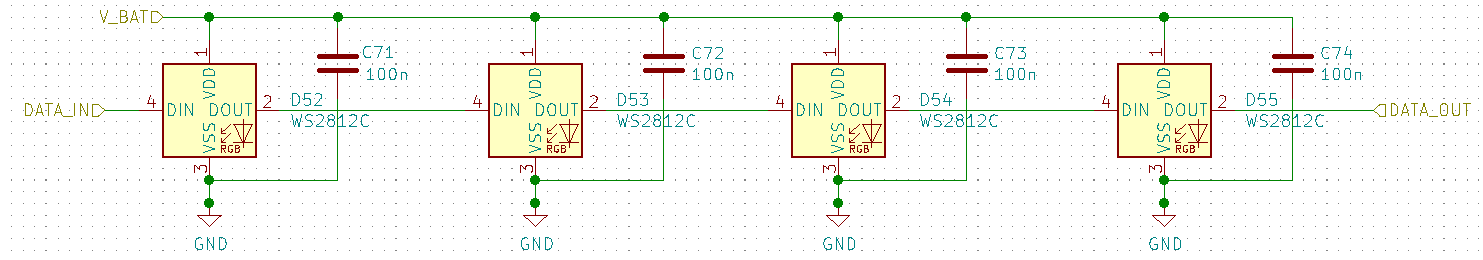
\includegraphics[scale=0.5]{obrazky/WS2812C_spojeni.png}
    \end{center}
    \caption[WS2812C spojení]{Zapojení LED WS2812C \cite{WS2812C_datasheet}.}
\end{figure}

Parametry LED WS2812C \cite{WS2812C_datasheet}: %přidat
\begin{itemize}
    \item Napájecí napětí 3,5 - 5,3 V,
    \item výstupní napětí -0,5 - VDD - 0,5 V,
    \item typický odběr proudu 5 mA,
    \item 
\end{itemize}

Porovnání WS2812C s WS2812B:
%tabulka

Ke každé LED je připojen na napájení filtrační kondenzátor \cite{WS2812C_datasheet}, aby LED svítili kontinuálně a nedostal se 
jim na napájení žádný šum.

\subsection{Rozdělení}
LED jsou rozděneny do tří skupin. Skupina LED pro zadání, skupina LED pro herní pole a skupina LED pro zobrazení vyhodnocení 
tahu.
Skupina LED pro zadání obsahuje 4 LED a skupiny pro herní pole a pro vyhodnocení každá 40 LED.

\section{Zapínání napájení LED}
DPS je navrhována pro přenosnou aplikaci, a proto je potřeba zajistit její co nejnižší odběr. 

LED mají určitou spotřebu, i když zrvona nesvítí žádnou barvou. Proto je herní pole dohromady s vyhodnocovacími LED rozděleno 
na 3 části. Do první části patří LED se zadáním a první 4 čtveřice LED z herního pole a z vyhodnocení. Do druhé části patří 
další 3 čtveřice LED z herního pole a z vyhodnocení. Do třetí části patří poslední 3 čtveřice LED z herního pole a z 
vyhodnocení.

Těmto 3 částem je postupně zapínáno napájecí napětí. Každé části se zapne napájení až pokud se hráč dostane do fáze, kdy 
danou oblast bude potřebovat. K zapínání dochází softwarově spínáním GPIO pinem procesoru.

Ke spínání slouží obvody s MOSFET tranzistory. MOSFET tranzistory byly zvoleny pro jejich nulovou spotřebu, narozdíl od 
bipolárních tranzistorů. 

\begin{figure}[!h]
  \begin{center}
    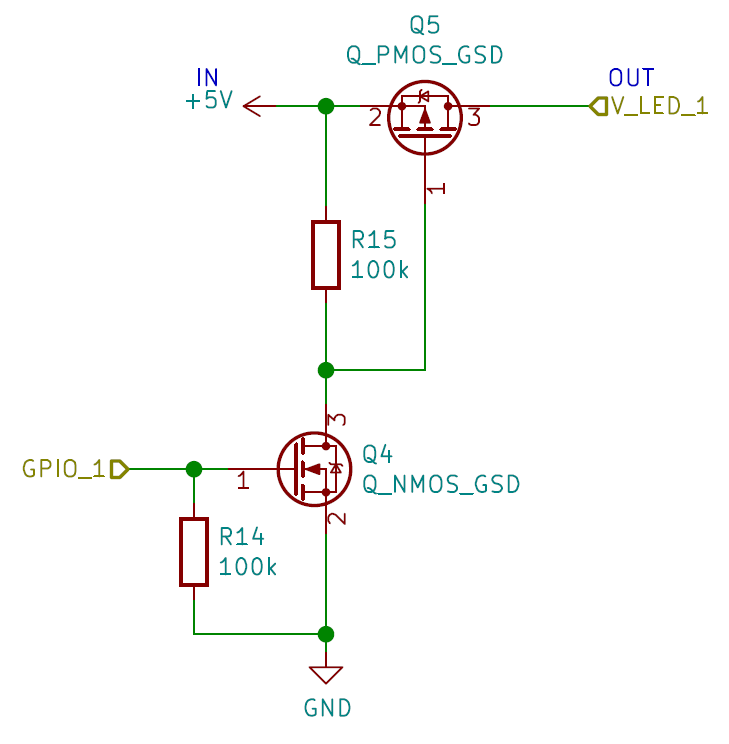
\includegraphics[scale=0.5]{obrazky/Zapinani_napajeni_LED.png}
  \end{center}
  \caption[Zapinani LED]{Obvod pro zapínání napájení pro LED.}
\end{figure}


\subsection{Popis funkce zapínání LED}
%přepsat

\section{Spínací prvky}
Přepínač SW1 slouží pro zapínání celé DPS. Tento přepínač připojuje napájecí napětí 5 V z USB k celému zbytku DPS.

Tlačítka slouží pro ovládání hry. Ke každému tlačítku je připojen kondenzátor o hodnotě 100 nF. Tento kondenzátor 
slouží pro filtraci zákmitů při zmáčknutí tlačítka. Filtrace se proto nemusí řešit softwarově.

\begin{figure}[!h]
  \begin{center}
    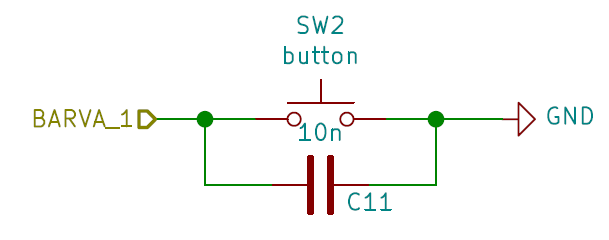
\includegraphics[scale=0.5]{obrazky/Tlacitka_zapojeni.png}
  \end{center}
  \caption[Zapojení tlačítek]{Zapojení tlačítek.}
\end{figure}

\section{PowerLED}
Diody D1 a D2 slouží pro indikaci přítomnosti napájecího napětí.  Dioda D1 indikuje přítomnost napájecího napětí 
5 V a dioda D2 indikuje přítomnost napájecího napětí 3,3 V.

\begin{figure}[!h]
  \begin{center}
    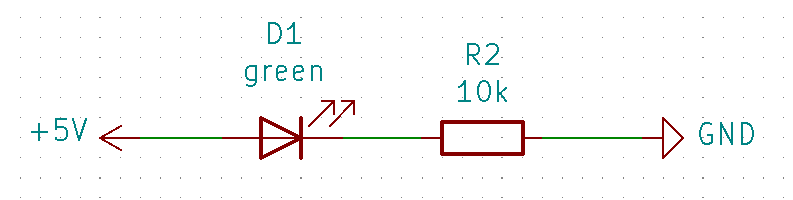
\includegraphics[scale=0.5]{obrazky/powerLED.png}
  \end{center}
  \caption[Zapojeni powerLED]{Zapojení LED pro indikaci napájecího napětí.}
\end{figure}

\chapter{Popis DPS}
DPS je navržena v programu KiCad a její parametry jsou určeny pro výrobu i osazení ve firmě JLCPCB \cite{JLCPCB}. Výrobní 
podklady proto musely být navrženy v souladu s jejich výrobními možnostmi \cite{JLCPCB_Capabilities}.

DPS má 4 vrstvy. Vnitřní vrstvy slouží pro napájení a vnější pro signálové dráhy. V jedné vnitřní vrstvě je po celé její ploše 
rozlité GND a ve druhé vnitřní vrstvě jsou rozlitá jednotlivá napájecí napětí.

Na vrchní straně jsou umístěny i plošky pro osazení SMD součástek, protože firma JLCPCB osazuje pouze SMD součástky z jedné 
strany. THT součástky jsou připraveny na ruční pájení.

Signálové dráhy jsou vedeny tenkou dráhou a napájecí dráhy jsou vedeny tlusčí dráhou. V signálových drahách tečou zanedbatelné 
proudy, proto mohou být co nejtenčí. Výrobce umožňuje vyrobit nejtenčí dráhu u čtyřvrstvé DPS 0,09 mm \cite{JLCPCB_Capabilities}. 
Aby nebyly použity krajní hodnoty, byla zvolena šířka signálové dráhy 0,150 mm.

Kondenzátoty u procesoru ESP32-PICO a u čipu CP2102 musí být umístěny co nejblíže jejich pouzdru. Tyto kondenzátory slouží pro 
filtraci šumu na napájení.

Dráhy od USB k čipu CP2102 D+ a D- fungují jako diferenciální pár. Proto musejí být jejich dráhy vedeny vedle sebe a blízko u 
sebe.

Rozložení počástek k čipu SY8105 na DPS může velmi ovlivnit jeho funkčnost. Rozložení a zapojení stepdownu 
bylo převzato z datasheetu.

\begin{figure}[!h]
  \begin{center}
    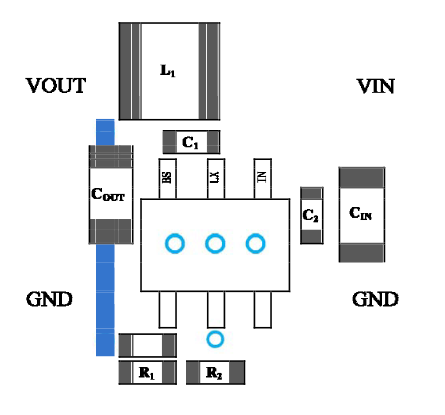
\includegraphics[scale=0.5]{obrazky/SY8105_rozlozeni_na_DPS.png}
  \end{center}
  \caption[SY8105 rozložení na DPS]{Rozložení součástek kolem čipu SY8105 na DPS \cite{SY8105_datasheet}.}
\end{figure}

LED jsou rozděleny do 3 skupin, aby se hra co nejvíce podobala deskové hře. LED pro zadání jsou v horní části DPS. V levém 
sloupci pod zadáním jsou LED, které slouží jako herní pole, a v pravém sloupci jsou LED pro vyhodnocení tahu. Každá LED musí 
mít svůj filtrační kondenzátor na napájení co nejblíže svému pouzdru.

\chapter{Oživení DPS}
\section{v0.0}
Po dodání DPS z výroby byly zapájeny THT komponenty (pouzdro na baterii, USB konektor, tlačítka a vypínač). Po zapojení baterií
18650 do pouzdra se rozsvítí zelená LED D1, která indikuje přítomnost napájecího napětí. Po připojení k počítači přes USB
se rozsvítí LED D9. Ta signalizuje nabíjení baterií. Pokud se rozsvítí LED D8, znamená to, že baterie jsou nabité.

\section{v1.0}
DPS přijde z výroby ve stavu, kdy jsou osazeny pouze SMD komponenty. % fotka DPS

Poté je nutné ručně osadit THT součástky, tj. vypínač, tlačítka a konektor USB micro. Připojení DPS přes USB k powerbance, 
nebo do počítače, se rozsvítí LED D1 a D2, které indikují přítomnost napájecího napětí. LED D2 zároveň značí, že stepdown je 
funkční.

\chapter{Způsob ovládání elektronické hry}
První verze je připravena jako hra pro jednoho hráče.

Po zapnutí DPS stikneme tlačítko "Nová hra". V této chvíli se vygeneruje zadání, které není vidět,
a na první herní LED se rozbliká kurzor. 
Kurzorem lze pohybovat pomocí tlačítek "Šipka vpravo" a "Šipka vlevo". Barvy LED se nastavují tlačítky ve spodní části DPS,
které jsou barevně označené. 
Po ukončení tahu stiskneme tlačítko "Potvrdit tah". Proběhne vyhodnocení a zobrazí se na vyhodnocovacích LED. Kurzor se posune
na první LED v dalším řádku.
Po zadání správné kombinace barev a jejich pozic se rozsvítí zadání a hra je u konce. Pro novou hru stiskneme tlačítko
"Nová hra" a pro ukončení tlačítko "Konec".
Při stisku tlačítka "Konec" zhasnou všechny herní, vyhodnocovací LED i LED pro zadání. Poté je DPS připravena pro vypnutí
vypínačem. V této fázi lze zároveň stisknout tlačítko "Nová hra". 













%možná vůbec nebude, nebo bude určitě jinde
\section{Nabíjecí obvod}
Pro nabíjecí obvod byl zvolen čip TP4056. Jeho zapojení bylo převzato z datasheetu [citace]. %tady bude obrázek schématu asi
Velikost rezistoru $R_\textind{PROG}$ se volí podle nabíjecího proudu. 
Tabulka rezistorů $R_\textind{PROG}$.. [citace]

\begin{table}[!h]
    \caption{Nastavení nabíjecího proudu rezitorem $R_\textind{PROG}$}
    \begin{center}
        \begin{tabular}{|c|c|}
            \hline
            $R_\textind{PROG}$ [kOhm] & Nabíjecí proud [mA] \\
            \hline
            10      & 130 \\
            \hline
            5       & 250 \\
            \hline
            4       & 300 \\
            \hline
            3       & 400 \\
            \hline
            2       & 580 \\
            \hline
            1,66    & 690 \\
            \hline
            1,5     & 780 \\
            \hline
            1,33    & 900 \\
            \hline
            1,2     & 1000 \\
            \hline
        \end{tabular}
        
    \end{center}
\end{table}

Nabíjení baterií by mělo probíhat při 0,5C, tudíž pro 18650 je to cca 0,5 A. Proto byl zvolen rezitor Rprog 2 kOhm.
